\section{Experiments}
\label{sec:experiments}

We study three two-dimensional incompressible-flow systems with Reynolds number as the parameter: flow past a circular cylinder, flow past a centered square cylinder, and the fluidic pinball. Each dataset spans steady, Hopf-onset, and periodic behavior. Errors $E_u$ and $E_p$ are relative field errors in percent, averaged using the protocol of each benchmark; $E_{\rm joint}=E_u+E_p$ where reported. ``Divergent'' denotes a rollout that does not remain finite under the original evaluation rule. We preserve the numerical values and held-out partitions of the journal experiments.

\begin{table}[t]
\centering
\caption{Benchmark and held-out autonomous-rollout protocol. Entries list train/validation/test trajectories by local chart.}
\label{tab:benchmark_summary}
\small
\setlength{\tabcolsep}{3.2pt}
\begin{tabular}{lccc}
\toprule
Benchmark & $S$ chart & $H$ chart & $P$ chart \\
\midrule
Circular cylinder
 & 20.0--46.4; 14/2/4; $K{=}56$
 & 45.5--59.2; 29/2/3; $K{=}56$
 & 57.3--200; 53/6/4; $K{=}48$ \\
Centered square
 & 50--95.4; 60/5/4; $K{=}16$
 & 94--102; 23/6/5; $K{=}48$
 & 98.5--150; 27/6/4; $K{=}24$ \\
Fluidic pinball
 & 10--19; 37/8/7; $K{=}56$
 & 16.6--25; 39/8/7; $K{=}56$
 & 21.25--60; 47/9/9; $K{=}32$ \\
\bottomrule
\end{tabular}
\end{table}

\subsection{Do local specialists support long autonomous rollouts?}

On the circular cylinder, the proposed specialists remain finite across every evaluated regime. In the steady regime, their velocity-error range is $0.0330$--$0.1723\%$, compared with $0.0384$--$0.2995\%$ for a vanilla learned specialist and $0.0845$--$0.3404\%$ for the global model. In the Hopf regime the vanilla model is not evaluable, while RAL-MoE-ROM gives $E_u=0.0032$--$0.0288\%$ and $E_p=0.0355$--$0.4321\%$. In the periodic regime it improves the velocity-error range over vanilla from $1.0393$--$3.0836\%$ to $0.3809$--$1.3473\%$. Full pressure ranges and the data-only ablation are in Appendix~\ref{app:circular}.

The centered-square specialists transfer the construction to a different geometry and mesh. Aggregate held-out errors are $(E_u,E_p)=(1.5311,1.4583)\%$ for the steady chart, $(0.4387,0.4844)\%$ for Hopf, and $(0.9395,1.0921)\%$ for periodic flow. On fluidic pinball, the comparison in Table~\ref{tab:pinball_autonomous} shows that the learned specialist removes the divergent rollouts of the projected baseline in the steady and Hopf settings and substantially reduces joint error across all four evaluations. This is empirical long-horizon evidence under the tested distributions, not a guarantee of stability outside them.

\begin{table}[t]
\centering
\caption{Fluidic-pinball autonomous prediction. Errors are percentages; ``div.'' counts divergent evaluation windows.}
\label{tab:pinball_autonomous}
\small
\setlength{\tabcolsep}{3.5pt}
\begin{tabular}{llrrrr}
\toprule
Regime ($K$) & Model & $E_u$ & $E_p$ & $E_{\rm joint}$ & div. \\
\midrule
Steady (56) & POD--Galerkin & -- & -- & -- & 448/448 \\
            & RAL-MoE-ROM & 0.2247 & 0.7593 & 0.9840 & 0 \\
Hopf (56)   & POD--Galerkin & 0.4378 & 48.50 & 48.94 & 141/320 \\
            & RAL-MoE-ROM & 0.0995 & 1.986 & 2.085 & 0 \\
Periodic (32) & POD--Galerkin & 1.641 & 41.56 & 43.20 & 0 \\
            & RAL-MoE-ROM & 0.2897 & 0.5518 & 0.8415 & 0 \\
Periodic core (56) & POD--Galerkin & 2.555 & 39.36 & 41.91 & 0 \\
            & RAL-MoE-ROM & 0.6222 & 1.050 & 1.672 & 0 \\
\bottomrule
\end{tabular}
\end{table}

\subsection{Does learned physical-space fusion improve overlap prediction?}

Table~\ref{tab:routing_fusion} separates hard routing from field-space combination on the centered-square benchmark. T2-C improves E2 Top-1 in both overlaps and is close to the a posteriori window-wise convex oracle. Equal weights and direct E2-probability weights do not reproduce the gain, indicating that the improvement is not a generic consequence of averaging. At $Re=95.1$, T2-C reduces joint error from $1.7140\%$ to $1.1827\%$; at $Re=100.5$, it reduces $2.6485\%$ to $0.8571\%$. Figure~\ref{fig:square_overlap} shows the corresponding physical fields and velocity-error maps. The complete parameter-wise table and fluidic-pinball overlap study appear in Appendices~\ref{app:square} and \ref{app:pinball}.

\begin{table}[t]
\centering
\caption{Centered-square routing and fusion at $K=24$. Lower is better.}
\label{tab:routing_fusion}
\small
\setlength{\tabcolsep}{4pt}
\begin{tabular}{llrrr}
\toprule
Overlap & Predictor & $E_u$ & $E_p$ & $E_{\rm joint}$ \\
\midrule
$S$--$H$ & E2 Top-1 & 0.4942 & 1.2356 & 1.7298 \\
          & Equal blend & 1.3644 & 1.6677 & 3.0321 \\
          & E2-probability blend & 0.7898 & 1.3949 & 2.1847 \\
          & T2-C & \textbf{0.4615} & 0.7343 & \textbf{1.1958} \\
          & Convex oracle & 0.4659 & \textbf{0.7183} & 1.1842 \\
\midrule
$H$--$P$ & E2 Top-1 & 0.7422 & 1.1052 & 1.8473 \\
          & Equal blend & 0.6077 & 1.0069 & 1.6146 \\
          & E2-probability blend & 0.6154 & 1.0464 & 1.6618 \\
          & T2-C & 0.4509 & 0.3956 & 0.8465 \\
          & Convex oracle & \textbf{0.4479} & \textbf{0.3905} & \textbf{0.8384} \\
\bottomrule
\end{tabular}
\end{table}

\begin{figure}[t]
\centering
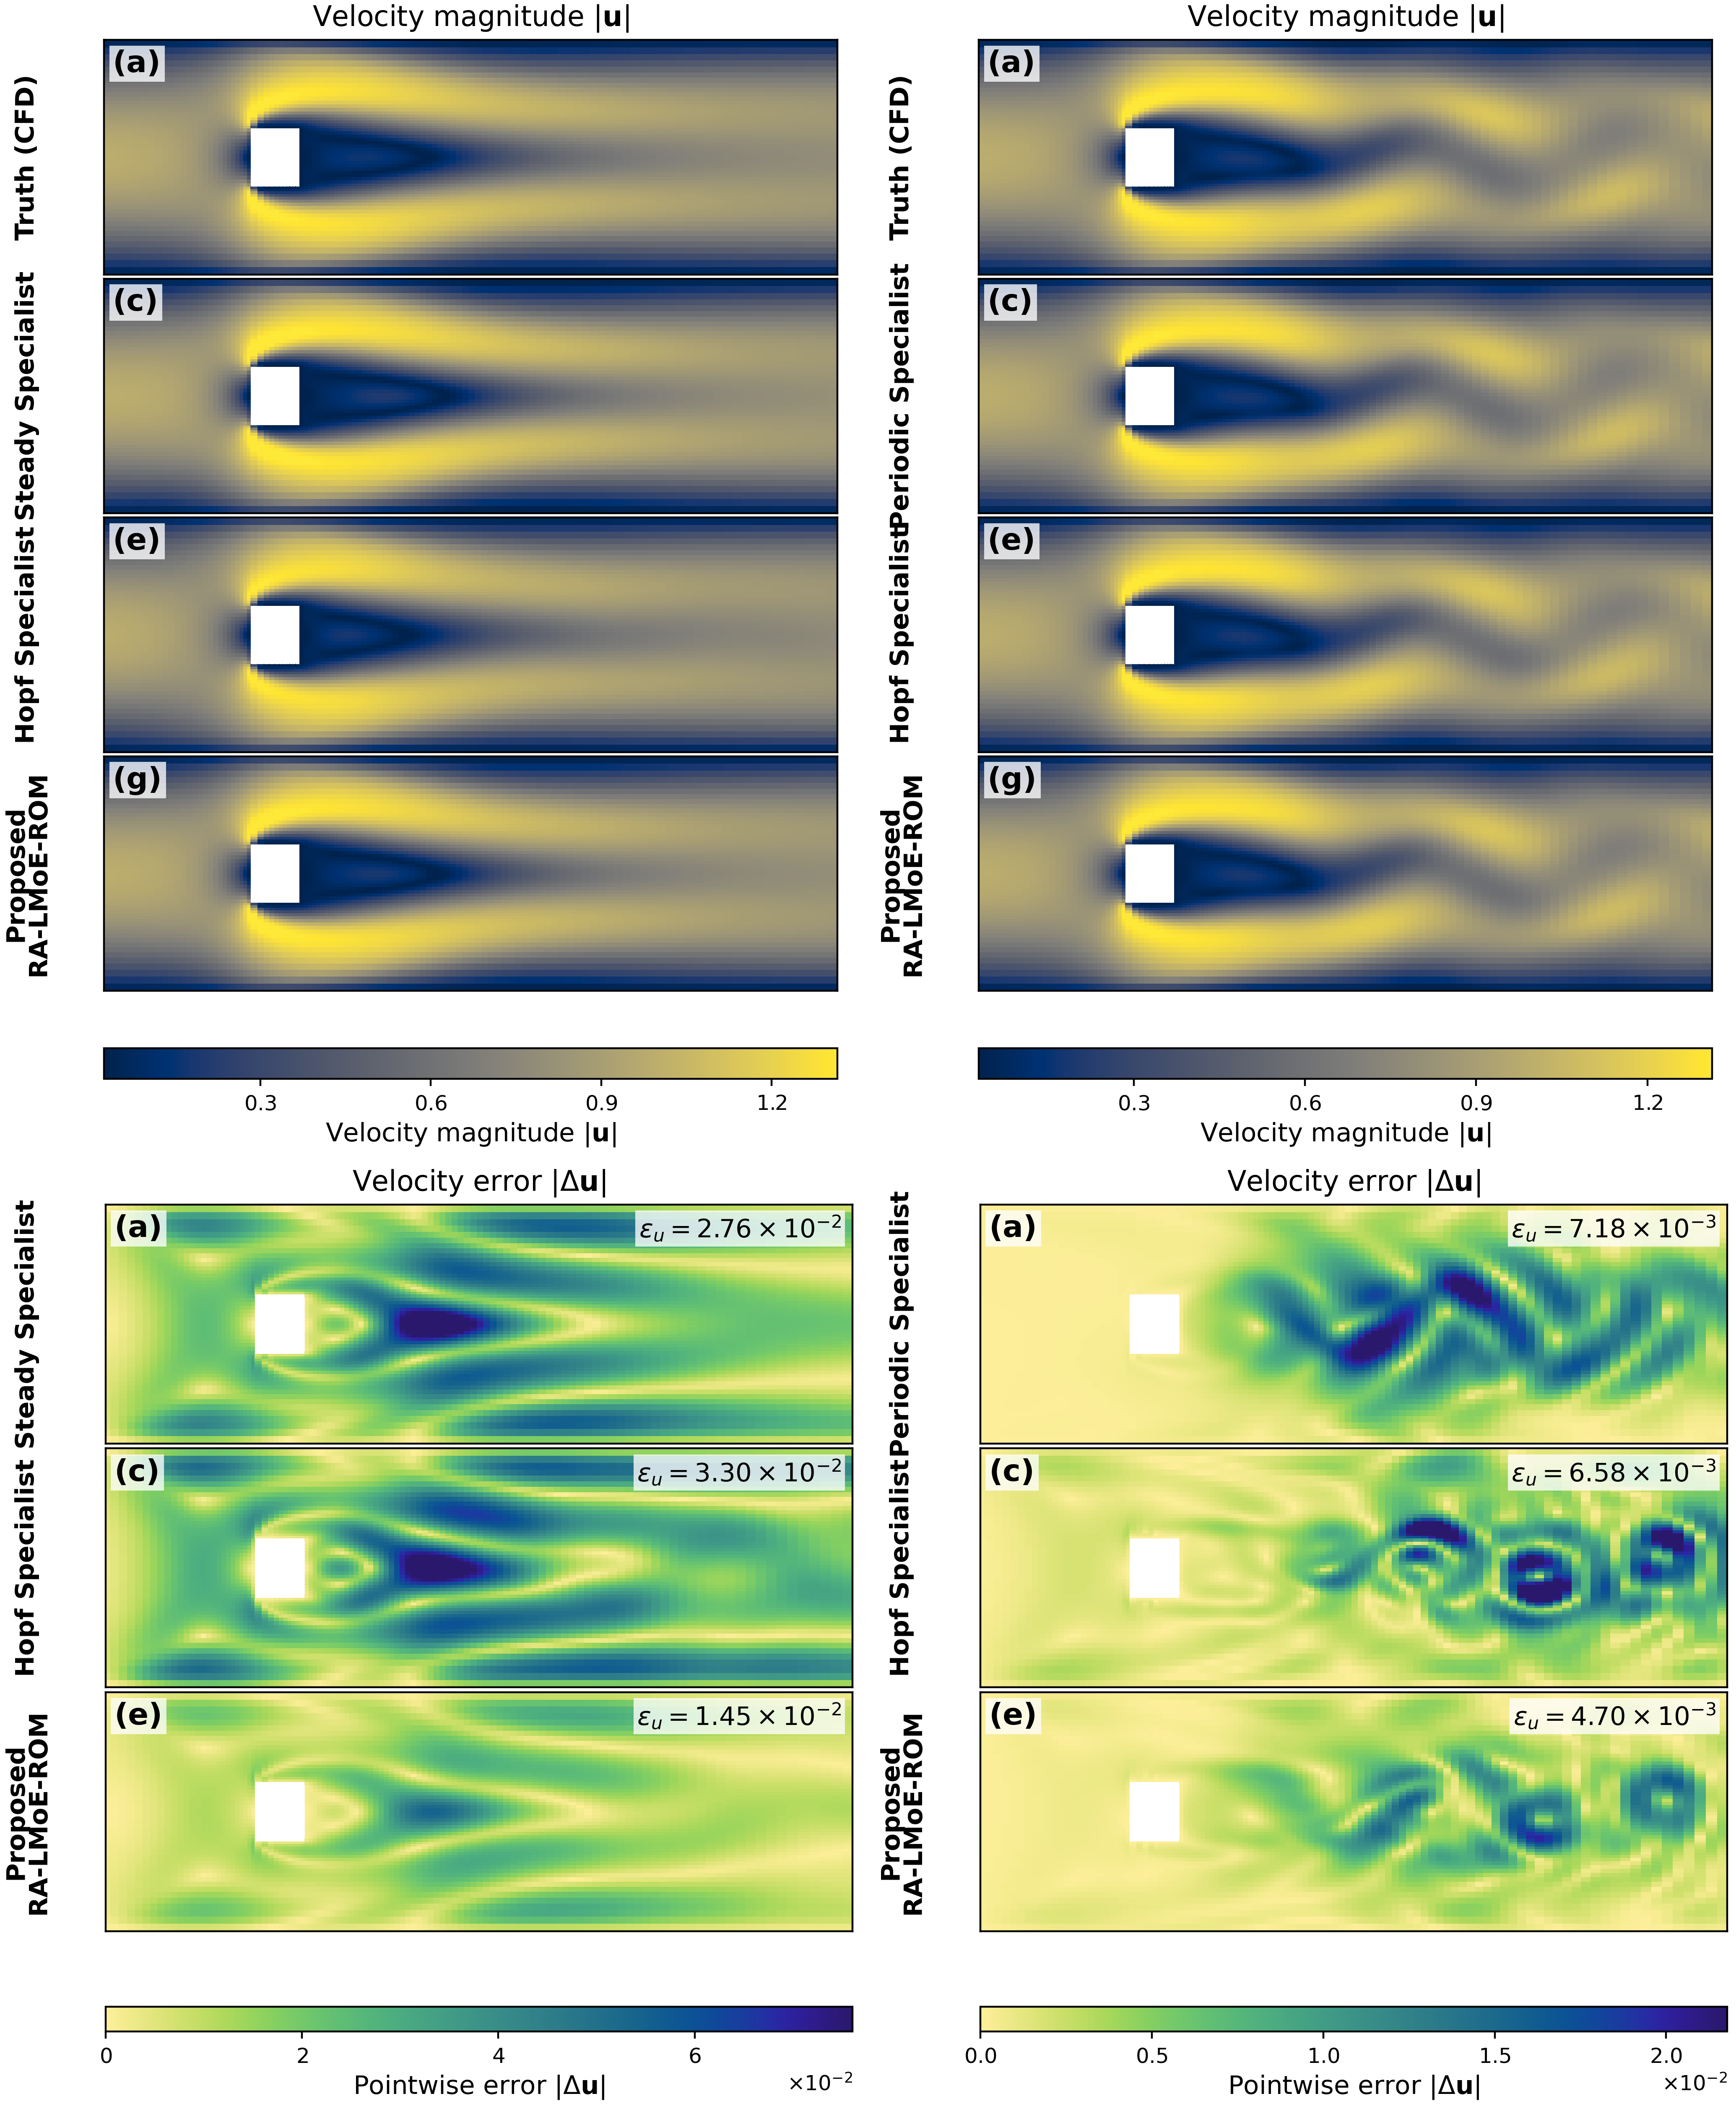
\includegraphics[width=\linewidth]{figures/square_overlap_compact.png}
\caption{Centered-square overlap predictions. Left: $S$--$H$ at $Re=95.1$; right: $H$--$P$ at $Re=100.5$. The upper panels compare CFD, the two adjacent specialists, and RAL-MoE-ROM using velocity magnitude. The lower panels show the corresponding absolute velocity errors. The composite crops only the velocity columns from the original full velocity--pressure panels and preserves their native raster pixels.}
\label{fig:square_overlap}
\end{figure}

\subsection{What contributes to the result?}

The original ablations isolate four effects. Removing the projected backbone produces the data-only degradation visible on circular-cylinder rollouts; replacing localized specialists with one global model sacrifices regime-specific accuracy, although the global model can remain competitive at individual parameters; replacing structured sparse experts with the vanilla learned correction widens long-horizon errors and fails in the evaluated Hopf case; and replacing T2-C with Top-1, equal, or raw-probability fusion worsens overlap prediction. Together these results support the architectural decomposition rather than a claim that any single component is uniformly dominant.
